\chapter{Text To Speech}
\ifpdf
    \graphicspath{{Chapter4/Chapter4Figs/PNG/}{Chapter4/Chapter4Figs/PDF/}{Chapter4/Chapter4Figs/}}
\else
    \graphicspath{{Chapter4/Chapter4Figs/EPS/}{Chapter4/Chapter4Figs/}}
\fi
\textit{Nội dung chương 4 sẽ giới thiệu tổng quan về bài toán Text to Speech, mô hình hoạt động, các ứng dụng của Text to Speech, các vấn đề cần giải quyết của module Text to Speech trong một hệ thống trợ lý ảo và cách giải quyết các vấn đề đó. Chương 4 cũng sẽ giới thiệu về chức năng, cách cài đặt, cách sử dụng cũng như các ưu nhược điểm của các thư viện iSpeech và Google Text to Speech.}

\section{Tổng quan}
Text to Speech (TTS), hay còn gọi là hệ thống tổng hợp giọng nói,  là một lĩnh vực trong khoa học máy tính. Text to Speech nghiên cứu phương pháp tạo ra giọng nói nhân tạo từ văn bản. Giọng nói nhân tạo này được đánh giá dựa trên hai tiêu chí: mức độ tự nhiên và mức độ dễ nghe. Mức độ tự nhiên chỉ sự tương đồng về ngữ điệu của giọng nói tổng hợp với giọng nói con người. Mức độ dễ nghe đánh giá khả năng phát âm rõ ràng, và khả năng nghe hiểu của con người với giọng nói tổng hợp. Việc có quá nhiều ngôn ngữ trên thế giới, cộng thêm việc mỗi ngôn ngữ lại có nhiều ngữ điệu khác nhau tùy vùng miền đã đặt ra những thách thức không hề đơn giản cho các nhà khoa học.

Text to Speech đã được bắt đầu phát triển từ rất lâu trước đây và đã trải qua một quá trình cải tiến lâu dài. Có thể nói khởi nguồn của nó là mô hình bắt chước giọng nói người với năm nguyên âm (u, e, o , a, i), được phát triển vào năm 1779 bởi nhà khoa học người Đan Mạch Christian Kratzenstein tại viện hàn lâm khoa học Nga. Từ đó đến nay, sau nhiều năm phát triển cải tiến, hệ thống tổng hợp giọng nói đã có nhiều bước phát triển vượt bật, giọng nói tạo ra ngày càng giống với ngữ điệu người và hỗ trợ nhiều loại ngôn ngữ trên thế giới. Hiện nay, có rất nhiều công ty tham gia vào phát triển hệ thống Text to Speech, trong đó nổi bật là các công ty: Google, Microsoft, iSpeech, Amazon,...

\section{Mô hình hoạt động}
Một hệ thống Text to Speech thông thường bao gồm hai thành phần chính: front-end và back-end.
\begin{itemize}
\item Front-end, hay bộ phận tiền xử lý (Pre-processor), thực hiện ba nhiệm vụ chính. 
	\begin{itemize}
		\item Phân đoạn (Tokenization): là quá trình phân tích cấu trúc của đoạn văn. Quá trình này phân phia và đánh dấu văn bản thành từng từ, nhóm từ, mệnh đề, câu văn và đoạn văn.
		\item Chuẩn hóa (Normalization): là quá trình chuyển đổi các ký tự số, ký tự đặc biệt, viết tắt trong văn bản về dạng viết đầy đủ. Ví dụ "Dr"  sẽ được chuyển đổi thành "doctor". 
		\item Phân tích ngôn ngữ (Linguistic analysis): bao gồm phân tích hình thái học (Morphological analysis) để tìm ra cách phát âm tương ứng của từng từ và phân tích cú pháp (Syntactic analysis) nhằm hiểu cách diễn đạt hay nhấn mạnh của từ.
	\end{itemize}
\item Back-end, còn gọi là bộ phận tổng hợp âm thanh (Speech synthesizer). Nhiệm vụ của phần này là tổng hợp các thông tin từ front-end thành giọng nói ở dạng sóng âm thanh.
\end{itemize}
\begin{figure}[h]
    \centering
    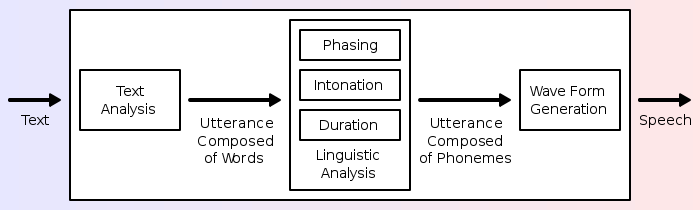
\includegraphics[scale=1]{ttsmodel}
    \caption{Minh họa mô hình hoạt động của hệ thống Text to Speech}
    \label{fig:c4_ttsmodel}
\end{figure}

\indent Có nhiều kỹ thuật dùng trong tổng hợp âm thanh. Tùy thuộc vào đặc tả của hệ thống, thiên về mức độ dễ nghe, thiên về mức độ tự nhiên, hay đồng thời cả hai tính chất trên mà sẽ lựa chọn kỹ thuật thích hợp. Có hai kỹ thuật chính thường được dùng là tổng hợp ghép nối và tổng hợp cộng hưởng tần số, ngoài ra còn có một số kỹ thuật khác.
\begin{itemize}
\item \textbf{Tổng hợp ghép nối}: Tổng hợp ghép nối dựa trên việc nối vào nhau các đoạn âm thanh của một giọng nói đã được ghi âm. Thông thường, tổng hợp ghép nối tạo ra giọng nói tương đối tự nhiên. Tuy nhiên, giọng nói tự nhiên được ghi âm có sự thay đổi từ lần phát âm này sang lần phát âm khác, và công nghệ tự động hóa việc ghép nối các đoạn của sóng âm thỉnh thoảng tạo ra những tiếng cọ xát không tự nhiên ở phần ghép nối. Có ba kiểu tổng hợp ghép nối.
\begin{itemize}
\item \textbf{Tổng hợp chọn đơn vị}: Tổng hợp chọn đơn vị dùng một cơ sở dữ liệu lớn các giọng nói ghi âm (thông thường dài hơn 1 giờ đồng hồ ghi âm). Trong lúc ghi âm, mỗi câu phát biểu được tách ra thành các đơn vị khác như: các âm tỏ lời đơn lẻ, âm tiết, hình vị, từ, nhóm từ, và câu văn. Thông thường, việc tách ra như vậy cần một máy nhận dạng tiếng nói được đặt ở chế độ khớp với văn bản viết tương ứng với đoạn ghi âm, và dùng đến hiển thị sóng âm và phổ âm thanh. Một bảng tra các đơn vị được lập ra dựa trên các phần đã tách và các thông số âm học như tần số cơ bản, thời lượng, vị trí của âm tiết, và âm tỏ lời gần đó. Khi chạy, các câu phát biểu được tạo ra bằng cách xác định chuỗi đơn vị phù hợp nhất từ cơ sở dữ liệu. Quá trình này được gọi là chọn đơn vị, và thường cần dùng đến cây quyết định để thực hiện.

Kỹ thuật chọn đơn vị tạo ra độ tự nhiên cao do không áp dụng các kỹ thuật xử lý tín hiệu số lên các đoạn giọng nói đã ghi âm, tuy rằng một số hệ thống có thể áp dụng xử lý tín hiệu tại các đoạn nối giữa các đơn vị để làm liền mạch kết quả sau khi ghép nối. Thực tế, các hệ thống chọn đơn vị có thể tạo ra giọng nói không thể phân biệt được với người thật. Tuy nhiên, để đạt độ tự nhiên cao, thường cần một cơ sở dữ liệu lớn chứa các đơn vị để lựa chọn; có thể lên tới vài gigabyte, tương đương với hàng chục giờ ghi âm.

\item \textbf{Tổng hợp âm kép}: Tổng hợp âm kép dùng một cơ sở dữ liệu giọng nói nhỏ chứa tất cả các âm kép (chuyển tiếp âm thanh) xuất hiện trong ngôn ngữ đang xét. Số lượng âm kép phụ thuộc vào đặc tính ghép âm học của ngôn ngữ: tiếng Tây Ban Nha có 800 âm kép, tiếng Đức có 2500. Trong tổng hợp âm kép, chỉ có một ví dụ của âm kép được chứa trong cơ sở dữ liệu. Khi chạy, lời văn được chồng lên các đơn vị này bằng kỹ thuật xử lý tín hiệu số như mã tiên đoán tuyến tính, PSOLA hay MBROLA.

Chất lượng của âm thanh tổng hợp theo cách này thường không cao bằng phương pháp chọn đơn vị nhưng tự nhiên hơn tổng hợp cộng hưởng tần số. Tổng hợp âm kép tạo ra các tiếng cọ xát ở phần ghép nối và đôi khi giọng nói kiểu robot do các kỹ thuật xử lý tín hiệu số gây ra. Lợi thế của phương pháp này là kích thước cơ sở dữ liệu nhỏ. Các ứng dụng thương mại của phương pháp này đang ít dần, tuy nhiên có nhiều hệ thống như thế này được phân phát tự do, và phục vụ cho nghiên cứu.

\item \textbf{Tổng hợp chuyên ngành}: Tổng hợp chuyên biệt ghép nối các từ và đoạn văn đã được ghi âm để tạo ra lời phát biểu. Nó được dùng trong các ứng dụng có các văn bản chuyên biệt cho một chuyên ngành, sử dụng lượng từ vựng hạn chế, như các thông báo chuyến bay hay dự báo thời tiết.

Công nghệ này rất đơn giản, và đã được thương mại hóa từ lâu, đã đi vào các đồ vật như đồng hồ biết nói hay máy tính bỏ túi biết nói. Mức độ tự nhiên của các hệ thống này có thể rất cao vì số lượng các câu nói không nhiều và khớp với lời văn và âm điệu của giọng nói ghi âm. Tuy nhiên các hệ thống này bị hạn chế bởi cơ sở dữ liệu chuyên ngành, không phục vụ mọi mục đích mà chỉ hoạt động với các câu nói mà chúng đã được lập trình sẵn.
\end{itemize}

\item \textbf{Tổng hợp cộng hưởng tần số}: Tổng hợp cộng hưởng tần số không sử dụng bất cứ mẫu giọng thật nào khi chạy. Thay vào đó, tín hiệu âm thanh cho ra dựa trên một mô hình âm thanh. Các thông số như tần số cơ bản, sự phát âm, và mức độ tiếng ồn được thay đổi theo thời gian để tạo ra dạng sóng cho giọng nói nhân tạo. Phương pháp này đôi khi còn được gọi là tổng hợp dựa trên quy tắc, dù cho nhiều hệ thống ghép nối mẫu âm thanh thật cũng có dùng các thành phần dựa trên quy tắc.

Nhiều hệ thống dựa trên tổng hợp cộng hưởng tần số tạo ra giọng nói nhân tạo, như giọng rôbốt, không tự nhiên, và phân biệt rõ ràng với giọng người thật. Tuy nhiên độ tự nhiên cao không phải lúc nào cũng là mục đích của hệ thống và hệ thống này cũng có các ưu điểm riêng của nó.

Hệ thống này nói khá dễ nghe, ngay cả ở tốc độ cao, không có tiếng cọ xát do ghép âm tạo ra. các hệ thống này hoạt động ở tốc độ cao, có thể hướng dẫn người khiếm thị nhanh chóng dò dẫm trên máy tính, bằng cách đọc to những gì hiện ra trên màn hình. Các hệ thống này cũng nhỏ gọn hơn các hệ thống ghép nối âm, vì không phải chứa cơ sở dữ liệu mẫu âm thanh lớn. Nó có thể dùng trong các hệ thống nhúng khi bộ nhớ và tốc độ xử lý có hạn. Hệ thống này cũng có khả năng điều khiển mọi khía cạnh của tín hiệu âm thanh đi ra, no cho ra một dải rộng các lời văn và ngữ điệu, và không chỉ thể hiện được câu nói thường hay câu hỏi, mà cả các trạng thái tình cảm thông qua âm điệu của giọng nói.

Các ví dụ về các hệ thống cho ra ngữ điệu chính xác (nhưng không cho ra ngay lập tức sau khi nhận đầu vào) là các công trình cuối những năm 1970 của đồ chơi Speak \& Spell của Texas Instruments, và các trò chơi video của SEGA đầu những năm 1980 như: Astro Blaster, Zektor, Space Fury, và Star Trek. Hiện vẫn chưa có hệ thống cho ra intonation chính xác ngay sau khi nhận văn bản đầu vào.

\item \textbf{Tổng hợp mô phỏng phát âm}: Tổng hợp mô phỏng phát âm là các kỹ thuật tổng hợp giọng nói dựa trên mô hình máy tính của cơ quan phát âm của người và quá trình phát âm xảy ra tại đó. Hệ thống tổng hợp mô phỏng phát âm đầu tiên là ASY, thường được dùng cho các thí nghiệm trong nghiên cứu, được phát triển ở phòng thí nghiệm Haskins vào giữa những năm 1970 bởi Philip Rubin, Tom Baer, và Paul Mermelstein. ASY dựa trên mô hình cơ quan phát âm đã được tạo ra bởi phòng thí nghiệm Bell vào những năm 1960 và 1970 bởi Paul Mermelstein, Cecil Coker, và các đồng nghiệp khác. Tổng hợp mô phỏng phát âm đã từng chỉ là hệ thống dành cho nghiên cứu khoa học cho mãi đến những năm gần đây. Lý do là rất ít mô hình tạo ra âm thanh chất lượng đủ cao hoặc có thể chạy hiệu quả trên các ứng dụng thương mại. Một ngoại lệ là hệ thống dựa trên NeXT; vốn được phát triển và thương mại hóa bởi Trillium Sound Research Inc, ở Calgary, Alberta, Canada. Đây là một công ty tách ra từ Đại học Calgary nơi các nghiên cứu ban đầu đã được thực hiện. Theo sau các vụ chuyển nhượng các từng phần của NeXT (bắt đầu từ Steve Jobs vào cuối những năm 1980 và việc hợp nhất với Apple năm 1997), phần mềm của Trillium được phân phát với giấy phéo tự do GPL. Dự án gnuspeech, một dự án của GNU, tiếp tục phát triển phần mềm này. Phần mềm gốc NeXT và các chuyển đổi sang cho Mac OS/X và GNUstep trong GNU/Linux có thể tìm thấy tại trang GNU savannah; chúng đều kèm theo tài liệu hướng dẫn trực tuyến và các bài viết liên quan đến lý thuyết nền tảng của công trình. Hệ thống, vốn được thương mại hóa lần đầu vào năm 1994, tạo ra một máy tổng hợp giọng nói dựa trên mô phỏng phát âm hoàn chỉnh, dựa trên mô hình ống dẫn sóng tương đương với cơ quan phát âm của người. Nó được điều khiển bởi Mô hình Phần Riêng biệt của Carré; bản thân mô hình này lại dựa trên công trình của Gunnar Fant và các người khác ở Phòng thí nghiệm Công nghệ Giọng nói Stockholm thuộc Viện Cộng nghệ Hoàng gia Thụy Điển về tổng hợp giọng nói cộng hưởng tần số. Công trình này cho thấy các cộng hưởng tần số trong ống cộng hưởng có thể được điều khiển bằng cách thay đổi tám tham số tương đồng với các cách phát âm tự nhiên của cơ quan phát âm của người. Hệ thống bao gồm một từ điển phát âm cùng với các quy tắc phát âm tùy thuộc ngữ cảnh để giúp ghép nối âm điệu và tạo ra các tham số phát âm; mô phỏng theo nhịp điệu và ngữ điệu thu được từ các kết quả nghiên cứu ngữ âm học.

\item \textbf{Tổng hợp lai}: Các hệ thống tổng hợp lai kết hợp các yếu tố của tổng hợp cộng hưởng tần số với tổng hợp ghép nối để giảm thiểu các tiếng cọ xát khi ghép nối các đoạn âm thanh.

Một ví dụ là RecSimCat, phát triển bởi Shakti Singh Parmar có thể tạo ra giọng dễ nghe và tự nhiên.[cần dẫn nguồn]

\item \textbf{Tổng hợp dựa trên HMM}
Tổng hợp dựa trên HMM là một phương pháp dựa vào mô hình Markov ẩn (HMM, viết tắt cho thuật ngữ tiếng Anh Hidden Markov model). Trong hệ thống này, phổ tần số của giọng nói, tần số cơ bản, và thời lượng đều được mô phỏng cùng lúc bởi HMM. Dạng sóng của giọng nói được tạo từ mô hình Markov ẩn dựa trên tiêu chí khả thực cực đại.
\end{itemize}

\section{Ứng dụng}
Hệ thống Text to Speech đang được nghiên cứu và ứng dụng trong nhiều lĩnh vực:
\begin{itemize}
	\item Máy đọc văn bản dùng cho những người mù chũ, có thị lực kém hoặc khiếm thị.
	\item Dùng trong ngành công nghiệp robot.
	\item Là công cụ giao tiếp của các trợ lý ảo.
	\item Trong luận văn này, hệ thống Text to Speech được sử dụng làm phương tiện để ứng dụng phản hồi lại lệnh của người dùng.
\end{itemize}

\section{Thư viện Google Text To Speech (gTTS)}
\subsection{Tổng quan}
gTTS là thư viện mã nguồn mở, được viết bằng ngôn ngữ python và hỗ trợ hoạt động trên đa nền tảng. Thư viện này được phát triển bởi Pierre Nick Durette một lập trình viên người Canada.
gTTS là một thư viện bao phủ trên nền Google's Text to Speech API cung cấp các tính năng giúp người dùng tương tác đơn giản hơn với hệ thống Text to Speech API của Google.

\subsection{Chức năng}
Thư viện gTTS có chứ năng chuyển một đoạn văn bản thanh giọng nói dưới dạng tập tin mp3. Thư viện này không giới hạn số từ của văn bản bằng cách chia đoạn văn bản ra thành các câu ngắn hơn tại các vị trí mà khi nói giọng người sẽ tạm ngừng một cách tự nhiên.

\subsection{Cách cài đặt}
\begin{itemize}
\item Windows, Mac OS, Linux: \lstinline[language=bash]{pip install gTTS}
\end{itemize}

\subsection{Cách sử dụng}
Thư viện gTTS có thể được sử dụng như là một python module hoặc chạy trên command line
\begin{itemize}
\item Python Module
\begin{lstlisting}
# Import gTTS
from gtts import gTTS

# Create an instance
 tts = gTTS(text='Hello', lang='en', slow=True)
#Parameters:
#text - String - Text to be spoken.
#lang - String - ISO 639-1 language code (supported by the Google Text to Speech API) to speak in.
#slow - Boolean - Speak slowly. Default False (Note: only two speeds are provided by the API).

#Write to a file
#To disk using save(file_name)
tts.save("hello.mp3")

#To a file pointer using write_to_fp(file_object)
f = TemporaryFile()
tts.write_to_fp(f)
# <Do something with f>
f.close()
\end{lstlisting}
\item Command line
\begin{lstlisting}[language=bash]
gtts-cli.py [-h] (["text to speak"] | -f FILE) [-l LANG] [--slow] [--debug] [-o destination_file]
$ # Example:
$ # Read the string 'Hello' in English to hello.mp3
$ gtts-cli "Hello" -l 'en' -o hello.mp3

$ # Read the string 'Hello' in English (slow speed) to hello.mp3
$ gtts-cli "Hello" -l 'en' -o hello.mp3 --slow

$ # Read the contents of file 'hello.txt' in Czech to hello.mp3:
$ gtts-cli -f hello.txt -l 'cs' -o hello.mp3

$ # Read the string 'Hello' from stdin in English to hello.mp3
$ echo "Hello" | gtts-cli -l 'en' -o hello.mp3 -
\end{lstlisting}
\end{itemize}

\subsection{Ưu điểm và nhược điểm}
\begin{itemize}
\item \textbf{Ưu điểm}: 
	\begin{itemize}
	\item Thư viện nhẹ, dễ sử dụng.
	\item Google's Text to Speech API hỗ nhiều nhiều ngôn ngữ, nhiều giọng đọc và cho ra giọng nói khá hay.
	\item Không giới hạn số từ của văn bản.
	\end{itemize}  
\item \textbf{Khuyết điểm}
	\begin{itemize}
	\item Chỉ có thể xuất ra tập tin mp3
	\item Không hỗ trợ stream âm thanh.
	\end{itemize}  
\end{itemize}

\section{iSpeech}
\subsection{Tổng quan}
iSpeech là một dịch vụ chuyển văn bản thành tiếng nói dưới dạng giao thức GET API. iSpeech được phát triển công ty iSpeech, một công ty được thành lập năm 2007 chuyên cung cấp các giải pháp về nhận diện tiếng nói và chuyển đổi văn bản thành tiếng nói.
iSpeech là một dịch vụ có thu phí, tuy nhiên công ty có cung cấp phiên bản demo miễn phí nhưng có nhiều giới hạn.

\subsection{Chức năng}
Chuyển đổi văn bản đầu vào thành tiếng nói dưới dạng tập tin mp3. Phiên bản demo của iSpeech giới giạn số từ tối đa trong văn bản là 36 từ.

\subsection{Cách cài đặt}
iSpeech là dịch vụ chạy hoàn toàn trên nền Web nên không cần bất cứ thao tác cài đặt nào.

\subsection{Cách sử dụng}
iSpeech được sử dụng bằng cách gửi request đến server bằng liên kết có dạng

\url{https://www.ispeech.org/p/generic/getaudio?action=convert&voice=usenglishfemale&speed=0&text=good+morning}

Trong đó:
\begin{itemize}
	\item \textbf{voice}:  tham số xác định giọng người đọc. iSpeech hỗ trợ hơn 30 giọng đọc với nhiều ngôn ngữ khác nhau. Xem thêm các giọng đọc khác mà iSpeech hỗ trợ \url{http://www.ispeech.org/api/#voices-standard}.
	\item \textbf{speed}: tốc độ đọc giá trị này nằm trong khoảng từ -20 đên 20.
	\item \textbf{text}: là văn bản cần chuyển thành tiếng nói. Các từ tỏng văn bản được nối với nhau bởi ký từ '+'.\
	\item Xem thêm các tham số mà iSpeech hỗ trợ \url{http://www.ispeech.org/api/#request-parameters}
\end{itemize}
\subsection{Ưu điểm, nhược điểm}
\begin{itemize}
	\item \textbf{Ưu điểm}:
	\begin{itemize}
		\item Giọng đọc rất giống với con người.
		\item Hỗ trợ stream giọng đọc trực tiếp từ server.
		\item Không cần cài đặt, dễ dàng sử dụng
	\end{itemize}
	\item \textbf{Nhược điểm}:
	\begin{itemize}
		\item Giới hạn 36 từ mỗi lần đọc.
		\item Giá của dịch vụ quá cao.
	\end{itemize}
\end{itemize}